\subsection{Goats}
\begin{figure}[htp]
    \centering
    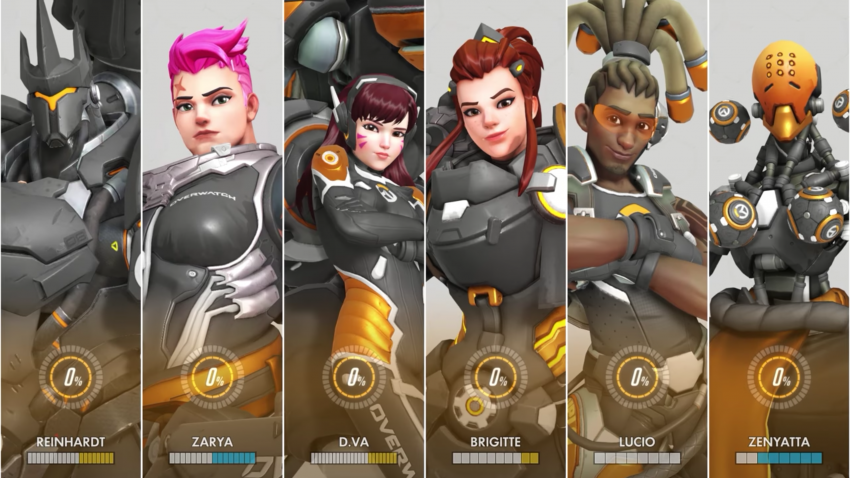
\includegraphics[width=0.8\textwidth]{figures/goats.png}
    \caption{고츠 조합의 기본 영웅들}
    \label{fig:goats}
\end{figure}
\subsubsection{introduction : 브리기테의 출현과 3탱3힐}\label{goats:intro}
오버워치는 4시즌(아나 루시우 젠야타 기용),5시즌(리메이크된 메르시,젠야타) 부터 거의 1년동안 윈디 다이브 조합이 유행하였다. 메르시와 젠야타의 유지력, 탱커들의 기동력과 여기 호응하는 겐지, 트레이서의 포커싱 때문에 원거리 영웅들이 안정적인 플레이를 하기 어려웠다. 이에 블리자드는 2018년 3월, 브리기테라는 새로운 지원가 영웅을 추가해 버티는 조합이 다이브 조합을 이길 수 있도록 만들었다. 당시 50이라는 방밀 데미지로 방밀캔슬을 활용하면 트레이서는 물론 200피 영웅까지 원콤보로 잡을 수 있었던 사기적인 데미지 뿐만 아니라, 600짜리 방패, 방어구를 채워주는 수리킷과 집결이 돌진조합의 핵심 딜량을 깎아버렸다. 게다가 집결을 다 받은 체력 200 영웅은 저격수의 헤드샷에도 죽지 않는 유지력을 보여주었다. 이 뿐만 아니라 방패를 넘어서 기절시키는 방패 밀쳐내기는 서로 라인하르트 대치 조합일 때 망치를 절대 막을 수 없게 만들었다.
이렇게 기존 딜러들 및 탱커들을 브리기테 하나가 전부 카운터해버리자, 아예 딜러를 빼버리고 함께 뭉쳐다니며 빠른 궁사이클과 부조화 포커싱으로 이득을 챙기는 3탱 3힐, 일명 고츠 조합이 등장하게 된다. GOATS!(팀 고츠) 에서는 루시우,모이라, 브리기테를 기용하는 3힐이었지만 여러 조합과의 상성을 고려하여 맞33전을 유리하게 가져가기 위한 루시우, 젠야타, 브리기테를 기용하는 3힐조합이 등장하게 된다.
고츠는 그 어떤 조합보다 케어용 스킬이 많고, 부조화를 이용한 포커싱이 중요하며, 궁사이클이 빠르다. 따라서 팀원들이 가지고 있는 자원을 어떤 순서로 사용할지, 상대의 자원을 어떻게 갉아먹을 수 있을지 팀원들 사이의 원활한 소통을 통해 계획해야 한다. 플레이어 개개인은 본인의 플레이가 팀파이트에 미치는 영향을 제대로 인지하고, 한타에서 본인의 역할을 정확하게 수행해야 한다. ioStux의 goats thesis\cite{ioStux} 를 참고하여 goats 조합의 운영법에 대해 알아보고, 2\-2\-2 조합이 고정된 현 시점에서 적용할 만한 포인트를 짚어보자.
\subsubsection{pre-fight}
궁극기 계산은 모든 한타마다 되어야 한다. 특히 한타 중에 차는 궁극기에 유의한다. 이는 어떤 조합이던지 당연하고, 위에서 설명했기 때문에 자세하게 언급하지는 않겠지만, 굳이 고츠에서 예를 들자면 상대 야타가 초월이 없고 아군 자리야가 자탄이 있다면 아군 자리야는 이 점을 무조건 인지해야한다. \\ 

한타가 시작하기 전에 아군의 자원 사용과 동선을 계획해야 한다. 미리 계획해두면 한타동안 소통의 부재로 일어나는 실수를 줄일 수 있으며, 어떤 궁을 이번 한타에 사용할 것인지 정하고 가야 한타중에 빠른 결정을 내릴 수 있기 때문이다. 한타 전에 계획할 대표적인 요소는 다음과 같다.
\begin{itemize}
    \item 비트 초월이 모두 있다면, 어떤 수비궁을 쓸 것인가?
    \item 어떤 공격궁(탱커궁) 을 사용할 것인가?
    \item 사용하려고 결정한 궁극기를 어느 용도로 사용할 것인가?
    \item 어느 타이밍에 어느 위치에서 그 궁극기를 사용할것인가?
    \item 어디서 홀딩할 것인가? 어디서 (어떤 상황에서) 뒤로 뺄것인가?
\end{itemize}
이를 조합하여 한타를 어떻게 진행할 것인지 계획한다.
\footnote{예를 들어 렐리가 있고, 상대가 막턴을 밟아야하는 상황이라고 해보자. 앞에서 빠르게 치고 들어가면서 앞라인싸움을 유도한다. 상대가 궁이 있고 아군의 카운터궁이 80정도라면 대치하면서 상대 중요 스킬이나 궁이 소모되도록 한다. 등등의 한타의 큰 그림을 그린다.}
 한타 전 계획이 익숙해질수록 지형적 특성과 궁극기 상황에 따라 팀원 개개인이 한타중에 취해야 할 행동을 쉽게 떠올릴 수 있게 된다. 즉, 팀원들간의 소통 없이도 상대의 어떤 약점을 캐치해내야 하는지, 어떤 궁에 대비해야 하는지, 그리고 어떤 궁을 사용해야하는지에 대한 판단이 암기된다. \\
한타 전 계획이 완료되었다면, 다음은 한타유도(initiating) 대해서 알아보자. 이 역시 팀원간 원활한 소통이 중요하다.

한타 중 팀원간 소통에서 주의할 점은 2가지가 있다.

 1. 소통은 언제나 직접적으로; 간접적으로 소통하는것은 고츠에서 최악의 선택임.
고츠의 기본은 속도다. 잘하는 팀은 상대로서 비집고 들어갈 구멍이 작기 때문에 그 작은 구멍을 붙잡고 버텨서 상대 수비를 열어야함. 
그러기 위해서는 팀으로서 확실한 결정을 내려야 할 필요가 있다. 고츠에서는 일단 지르고 그 다음에 생각을 해야한다
예를 들자면, 상대 자리야 자방이 빠졌을때, 저쪽 자방 빠졌으니까 들어갈래? 가 아닌 저쪽 자리야 자방 빠졌다 콜이 들림과 동시에 모든 팀원이 자리야를 포커싱.

 사람들이 하는 가장 큰 착각은 고츠에서 라인이 메인오더를 한다고 생각하는것이다.
하지만 고츠조합은 6명이 하나의 유닛으로서 움직이는게 제일 중요하며 고츠에서 한타 시작은 각각의 플레이어가 아닌 팀원 전체가 하나의 유닛으로 하는 것이다.
쉽게 말해서, 상대가 뇌절하면 누구 한명이 쟤네 누구 뇌절했다, 들어갈래? 가 아니라 팀원 6명 전부 상대가 뇌절했다는것을 인지하고 바로 이득을 봐야함.

Ex) 쟤네 자리야 주방 빠졌다, 라인 포커싱하자! =>ㅇ
     쟤네 자리야 주방 빠졌으니까 라인 노리는거 어때?=>x

 한타의 결과가 좋지 않다면 그것은 당신이 고츠를 이해하지 못하거나 팀원이 고츠를 이해하지 못한 것, 또는 당신의 팀원이 한타을 위한 준비가 안됬던 것이다 ex)포지셔닝,스킬쿨

 한타를 하려고 할때(본인이) 팀원중 누군가가 준비가 안되었다고 하거나 한타유도를하는 것을 거부한다면 그냥 "하지마!" 라고 빠르게 외치고 한타를 그만둬라.
한타를 한다는 콜을 특정 영웅이 하는 것이 아니라, 6명중 누구던지 콜을 할 수 있는것.
단, 6명 모두 한타에 대한 자신의 판단이 확실해야 하며, 판단이 확실하게 서지 않는다면 본인이 이유를 찾아야 한다( 위치선정, 낮은 이해도)

2. 고츠에서 모든 한타는 목표 영웅 하나를 정하고 해야함.
            주방빠졌다! 들어가!=>x
            주방빠졌다! 라인잡아!=ㅇ
명확한 대상없는 포커싱 오더는 팀의 분열을 부른다

 한타를 한다는 것은 상대의 중요한 스킬이나 상대의 위치가 안좋다는것이다. 
따라서 상대는 뒤로 빠지거나 산개하여 피해를 최소화하려고 할것이며,
확실한 목표를 설정하지 않고 한타를 한다면 팀원 6명이 서로 다른 영웅을 목표로 하고 움직이기 때문에 결과가 좋지 않을수밖에 없다.

3.포커싱 대상 호출(taget call)
 한타에 대한 콜을 너무 복잡하게 생각하지 마라.
가장 가까이 있는 영웅을 포커싱 한다는 콜은 아무 문제가 없다.  
허나 안좋은 결과를 만들수 있는 경우가 몇 가지 존재한다.
\begin{itemize}
    \item 상대 앞라인이 건재한 상태에서 그 뒷라인의 영웅을 포커싱 하자는 콜
    \item우리팀 본대에서 거리가 너무 멀리있는 상대팀 영웅에 대한 포커싱 콜
\end{itemize}
데미지 딜링이 신속히 이뤄져야 자리도 쉽게 먹을수 있다.

상대 자리야가 라인옆에붙어있다면 자리야 콜이 맞지만, 거리가 좀 멀다면 우리쪽의 포지션이 무너진다.
자리야에게 이동하다가 라인과 브리기테를 상대해야한다는 것을 보는 순간 자리야 포커싱을 중지하라는 콜을 팀에게 전달하여 멈추는 것이 좋다.
완벽한 타겟을 잡으려고 우리팀의 포지션을 희생하는거 보다 그 타켓을 잡는것을 포기하고 우리의 포지션을 완벽하게 잡는게 더 좋다.

고츠가 특이한점은 누가 콜을해도 이상하지 않다는것이다
돌진조합에서는 윈스턴이 콜을 해야하지만 고츠에서는 라인이 콜하던 자리야가 콜하던 차이가 없음.
글쓴이(ioStux,XL2 코치)의 경우 팀내에서 말이 제일 많고 목소리가 제일 큰사람을 주로 콜 하게 함.
콜을 주로 하는 사람을 팀내에서 정할때는 실험적으로 해도 된다.
특정 영웅을 플레이한다고 메인 콜을 하게 하는 것은 잘못된것.

그러나 콜하는것에 강약조절은 필요하다
목소리가 언제나 크고 말이 언제나 많은 사람이 자잘한 브리핑까지 맡는것은 효율이 떨어짐
정보 전달은 침착하게 해야하며 긴급한 브리핑은 큰소리로 빠르게 해야한다

한타 설계를 실행 할수 있는 것. 그런 강약 조절과 소통이 되어야 완벽하게 한타를 할 수 있다
따라서 자잘한 브리핑을 서로 완벽하게 하는게 중요함. 팀원 모두에게 똑같은 정보가 머리속에 입력되어있는게 제일 이상적.

---명확한 오더 및 한타 중 계획----
마지막으로 소통에 대해 언급하고자 하는 점은 한타 중 계획이다.
한타 전 설계는 매우 중요하지만 한타를 하다보면 계획이 변경될것이다.
서로 고츠조합에 익숙하지 않다면 한타가 오래 지속될것이다.
이럴 경우 한타중에 궁이 예상치 않게 차게 되는 경우가 존재한다(우리팀이든 상대팀이든)

한타전 계획이 미숙하다면 한타중에 차게되는 궁을 연계하기가 어렵다
따라서 브리핑이 활발해야한다
글쓴이의 경우 어떤팀을 잠깐 피드백 했었는데 
그팀은 시도때도 없이 나이스만을 외쳐되서 필요한 브리핑이 전혀 이루어지지 않았다
그런 상황을 방지하기 위해 중요한 내용을 신속하고 침착하게 브리핑 하는것이 중요하다

한타 전 설계를 잘해놓고도 한타 도중에 타겟설정이나 궁 사용에 대한 적절한 소통이 이루어지지 않아
궁을 낭비하거나 포커싱이 흐트러지거나 중요 궁을 너무 아껴 결론적으로 망한다거나 하게 된다
고츠 메타에서 소통은 연속적이여야 하며, 쉬어가는 타임은 없다는 것을 인지해야한다.

고츠조합에서는 한타의 목표가 무조건 상대궁이 빠지도록 유도하는 것은 아니다.
고츠조합에서의 목표는 상대가 뇌절또는 실수하도록 하는 것이기 때문에, 너무 대놓고 궁극기로만 플레이하면 상대가 실수를 하지 않기때문에 목표와 어긋난다
물론 예외는 있다 (6궁 vs 야타 노초월)
또는 추가시간 마지막한타
예를 들면, 왕의길 2거점 화물길은 ㄱ자 길이 많기 때문에 대놓고 자탄자폭콤보로 빠르게 막는것은 오히려 상대방이 한턴 져주고 
리그룹을 빠르게 할 수 있기때문에 효율성을 잘 따져봐야 한다.
한타를 이기고 궁 게이지를 조금 앞서는 것이 한타를 완벽하게 이기고 궁게이지가 바닥나는거 보다 좋다

기본적인 한타유도 3가지
\begin{itemize}
    \item 고지대 한타유도 : 우리팀이 수비중일때 상대방이 고지대를 먹고 내려오려고 할때, 간단하게 가장 먼저 고지대에서 밑으로 내려오는 상대 영웅을 포커싱한다. 예를 들어 리장타워 야시장 맵의 경우, 상대방이 좁은 1층에서 자리싸움을 꺼려하여 2층으로 돌아서온다면, 고츠를 못하는 팀일수록 1층으로 내려오는 속도가 영웅마다 다르다. 주로 라인이 먼저 내려오게됨. 이럴때 라인을 포커싱하여 죽이던가, 상대방의 스킬이 라인을 살리는데 빠지는 상황을 노려 이득을 챙긴다. 또는 상대방이 고지대에 있으면 디바 부스터나 루시우 밀치기로 한명을 떨어트리고 포커싱하는 것도 방법이 된다.
    \item 따로 떨어진 영웅 포커싱 : 상대 디바가 우리 야타를 잡으러 무리한다던지, 상대 브리기테가 본대와 멀어지는 실수를 하는 경우, 따로 떨어진 하나의 영웅을 포커싱하여 잡는다. 이것은 팀원 모두가 언제나 상대 포지션이 떨어져있는지 아닌지를 인지하고 있어야 한다. 앞라인에 주로 있는 라인 자리야 브리기테의 경우 뒤를 잘 못보기 때문에 본대 앞라인 뒤로 들어온 영웅들에 대한 콜을 뒷라인이 적극적으로 해줘야함. 2번의 경우 루시우의 이속 볼륨업이 무조건 필요한건 아니다.
    \item 자리야 주는 방벽 확인 : 상대 자리야 주방이 빠지고 우리는 주방이 있을때 한타를 시작 한다. 별개의 경우도 존재하지만, 90프로 이상의 상황에서는 3번 방법를 한다. 한타유도로 인해 킬이 나면 이상적이지만, 킬이 나지 않았다고 해서 실패인건 아니다. 조심해야 할 것은 한타유도를 한 후 우리팀의 스킬 쿨이 돌고있을때가 제일 위험하고 취약한 상황이다. 그 상황을 다른 스킬 등으로 잘 버티거나 넘기는 것이 좋은 팀이다. 부조화를 이용하는 한타유도도 가능하지만 실패할 리스크가 매우 높다. 자리야 자기방벽이 빠진상태에서 자리야 부조화 같은 경우는 좋은 시도가 될수 있다.
    \item Playing the line이라는 한타유도 방법이 존재 한다. 이는 특정 맵에 가상으로 줄을 그어 놓고 (주로 ㄱ자 길 또는 좁은 길)
대치상황에서 상대방 영웅 중 그 선을 넘은 영웅에게 포커싱을 가하는 하는 것이다.
좋은 예는 하나무라 a거점 수비측. 상대가 정문 조금 앞쪽 라인을 넘으면 6인이 전부 그 영웅을 포커싱.
또한 공격측에서 한명을 따고 거점 한칸을 먹은상태에서 상대가 재정비하고 다시 거점으로 한타하러 올때, 
공격측은 거점 두개의 문에 각각 줄을 그리고 그 선을 넘은 영웅을 어느쪽이든 포커싱.
Playing the line은 상대가 고츠를 잘하는 팀이면 성공률이 떨어진다.


\end{itemize}



레킹볼 3딜 방벽쪼개기 조합에는 2cp맵에서 고츠를 수비에 사용해 궁을 모으고 2거점에서 궁 사이클을 돌리며 막을수 있도록 쓸 수 있다. 단 2거점 입구가 상당히 좁아야 한다
이런경우 1거점에서는 한타유도 보다는 팀원 전원의 생존과 버티기를 위주로 수비한다
한타를 하는 경우는 언제나 상대방이 뇌절했을때
 - 타겟 정하기
한타유도로 첫 킬을 따낸 후 그다음 타겟을 정하는게 매우 중요하다.
첫킬 이후 상대 자리야가 근처에 있다면 자리야를 노리는게 제일 좋다.디바를 노리는 것은 좋지 않다. 고츠조합의 메인 딜 소스를 차단해버린다는 느낌으로 타겟을 잡아라.
특히 자리야는 도주기가 없기 때문에 첫킬 이후 타겟으로 정말 적합하다.

자리야 디바를 보기 어렵다면 라인의 방벽에 타겟을 잡아주자. 한타가 껄끄러워 질때쯤 상대 라인의 방벽이 관리가 안되게 된다--> 아군 대지분쇄로 한타 정리 가능.
도주기가 있는 대상은 타겟으로 왠만하면 잡지 않는것이 좋다. 갑자기 타겟이 없어져 팀의 한타에 비는시간을 만들기 때문
루시우를 한번에 죽일거 아니면 그 딜을 상대 라인 방벽에 꼬라박는게 더 낫다.



---기술---
-조화의 구슬
HPS(초당 힐량)는 단순히 HPS가 아니다. 체력을 3가지 단위로 구분하면 아머> 체력> 쉴드인데, 
따라서 이상적으로는 조화의 구슬을 아머가 존재하는 영웅에 달면 숫자로는 60의 데미지를 막을수 있는것.
이상적으로는 아머가 있는 영웅에게 조화의 구슬을 달면 2배의 효율을 낼 수 있지만, 실제로는 그렇지 않다. 하지만 효율이 더 올라가는것은 맞다.
아머가 이미 남아있는 영웅보다 아머가 없는 영웅이 더 체력적으로 약한것==> 따라서 조화의 구슬이 자리야에 달려있다면 
그것은 다른 관점으로 본다면 상대방이 아군의 라인하르트의 아머를 깎을수 있는 기회가 되는것
이는 아군 라인의 체력저하로 이어지며 아군 라인이 부담이 되 자리싸움에서 밀리거나 심각한상황에서는 죽게되는 상황까지 이를 수있게됨.
또는 수비형 스킬들이 빠지는 결과를 초래하게됨(자리야 주는방벽)
따라서 조화의 타겟팅은 한타 시작전에는 라인에 있는게 제일 이상적임.
또한 수준높은 라인하르트는 자신에게 조화가 고정되어있다는 생각을 하고 플레이를 할때가 많음.
다른 두 탱커영웅들은 브리의 힐량이나 루시우의 힐량정도로 생존이 가능하기때문에 조화는 왠만하면 라인에게 고정하는것이 정답,
또한 조화는 힐이 급할때 쓰기 보다는 지속적으로 달아놓는게 더 효율이 좋다. 예를 들어, 우리 자리야가 포커싱당하는데 거기다가 조화를 달아준다고 결과가 크게 달라지지는 않는다.
요점은 라인의 아머가 최대한 오래동안 남아있도록 조화를 고정해주는것. 고츠에서 위급한 상황에서의 힐은 브리의 수리팩이나 자리야의 주는방벽임.

-부조화의 구슬
부조화 메인 타겟팅은 상대 라인하르트가 되어야함. 야타 본인이 떄리는 대상이 라인이 아니더라도 가능하면 부조화는 라인에게 고정.
또한 부조화를 라인에 달음으로서 상대 자리야 주는방벽이 라인쪽으로 빠지도록 유도 후 다른 영웅을 포커싱하는 전법도 사용할 수 있게 된다.
상대 라인에게 부조화가 달리는 것 만으로도 엄청난 부담이됨.

-자리야 방벽
자리야 방벽을 잘못쓰는 것이 고츠 미러전에서 지는 가장 크고 잦은 이유이다.
자리야가 아군라인에게 방벽 원하는 타이밍 콜해달라는 것은 좋지 않음. 절대 하지 말것.
주는방벽 타이밍은 자리야 플레이어의 책임이 동반되어야한다.
라인에게 주방 콜 해달라는건 정말 하지말라고 강조하고있음.
자리야 본인이 알아서 타이밍 재서 쓰는게 가장 효율적.

중요한 것은 스킬을 마지막 순간까지 아끼는것.
가장 좋은 예는 자리야 방벽과 젠야타 초월.
늦게 쓸스록 이득을 많이 볼 수 있음.
허나 늦게 쓴다는건 팀원과의 믿음이 견고해야함.
타이밍 안맞으면 팀웍이 떨어지게됨.
스킬을 아끼는 것이 중요한 이유는 자리야 방벽의 경우 일종의 치킨게임이기떄문.
얼마나 이 치킨게임에서 우위를 점하느냐에 따라 상대 자리야에 우위를 점할 수 있음.
또한, 자리야 방벽을 이렇게 쓸 경우 브리기테 수리팩으로도 많은 이득을 볼 수 있음.
풀피 라인에 주방주는거는 딱 두가지경우에만 하도록 
1. 라인이 방벽이 다 꺠졌고 라인앞에 자폭이 있을떄 
2. 라인이 상대 라인에 돌진맞아 제압되어있을떄

그외에는 먼저 주방을 쓰는건 상대에게 한타를 시작할 타이밍을 주는 행위.
고츠에서는 사실 주는 방벽을 안써도 되게 상황을 만드는것이 정말 좋음.
거두절미하고 아군 라인이 상대쪽으로 풀피상태로 뛰어드는데 주방을 줬다면 그건 자리야가 게임을 던진거다. 주방은 긴급탈출버튼이다.
주방에 대한 상황은 4가지
1. 우리가 먼저쓰고 상대가 안씀. 
2. 저쪽이 먼저쓰고 우리가 안씀. 
3. 저쪽이 먼저쓰고 우리가 몇초 있다 쓴다. 
4. 우리가 먼저쓰고 저쪽이 몇초 있다 쓴다.

1상황: 절대 하면 안된다. 이런 상황이 벌어지는건 보통 조화가 라인에 고정이 안되있다거나 라인이 방벽을 제떄 안들어서 부조화맞고 압박당한다거나.
이런 상황이 벌어진다면 1순위 목표는 생존.
상대 자리야가 아군 주방이후 무조건 주방을 쓴다는 확신이 있으면 먼저 주방을 써라.

2상황: 이 경우 생각해볼수 있는 것은 다음 주방이 돌아올때 상대방 주방이 쿨타임이라는 것.
이런경우 보통 콜이: 저쪽 주방 썼고 우리 주방 곧 온다.. 3..2..1...
이 콜을 듣고 아군 모두는 본대가 한타를 유도하러 들어갈 것이라는 것을 인지해야한다.

3상황: 이것이 가장 좋은 방법이라고 할수 있다.
만약 이상황이 발생하면 적군팀의 오더나 브리핑을 꼬거나 힘싸움에 있어 많은것을 우리에게 유리하게 되도록 상요할수 있다.
자리야 방벽이 사라지자 마자 진입을 하면 된다 2~3초의 자리야 방벽으로 인한 이득보다 우리팀에게 싸움에서 이기기 충분한 8초의 시간을 줄수있다
그러나 이 상황이 발생하였을때 이기지 못한다면 이점이 사라지고 불이익이 발생할구 있다 상대는 우리의 실수를 유도 하기 위해 노력할 것이다
이 상황을 이용해 가장 큰 이득을 보려면 본인(자리야)의 자신감이 확실하고 젠야타의 구슬 고정을 확인하며, 상대 포커싱에 대한 오더가 일관되고 빠르게 진행되야 할것이다

4상황:가장 나쁘지는 않지만 좋지도 않다. 물론 먼저 주방을 사용하기 위해 적의팀을 시험하고 죽여야 하지만 다시 한타를 여는것에 대하여 신중해야 한다
우리팀이 아무도 죽이지 않고 목표(거점,화물)을 점거하고 있고 그들이 무엇을 하고 있는지를 안다면 주방 쿨타임이 돌기전에 상대팀이 우리를 죽이려 할것이다
우리가 주방을 먼저 주었을때 무언가를 죽일수 있다고 생각하지 않는다면 뒤로 빠져 다시 한타를 열어 중립적인 상황에서 다시 돌아온 주방 쿨타임을 이용해서 
한타를 열어야 할 것이다

이 4가지 상황을 모두 이해하는것이 중요하다,
팀원 모두가 이 4가지 상황 모두에서 할 일을 이해해야한다
누군가가 이 상황들을 식별하는데 어려움을 겪는다면
자리야가 방벽을 사용할때 오더와 브리핑에 있어 더 많은 점유율을 차지 하는것이 
도움이 될수 있다.

자리야가 일방적으로 이득을 취하는 방법은 적에게 과도한 궁사용을 유도해 다음 싸움을 압도하는 것이다.
이를 위해 방벽 훼이크(원문은 bating bubbles이나 이렇게 함)가 유용하다 이것은 적팀이 2상황에 들어가게 하는 것을 미끼로 하는 방법이다.
이것은 매우 간단하다 가짜 교전을 하고 아군 라인이 풀피일때 방벽을 사용하고 상대라인에게 압박을 넣는척 해라
이것은 상대를 죽이거나 공간을 차지할 목적으로 하는것이 아닌 상대가 우리팀이 뇌절한것 처럼 보이게 하여 궁극기를 사용하게 하는것이다.
이 과정에서 궁극기를 빼지 못하더라도 상대 주방의 쿨타임을 계산하여 4상황을 유도해 한타를 비등하게 가져갈수도 있다.

자리야에 대한 마지막으로 자탄 자폭에 대해 설명하고 이것이 방벽에 어떻게 영향을 미치는지 알아야한다
적이 자탄자폭을 가지고 있다면 초월은 일반적인 상황에서 의미가 없다
방벽이 라인을 방밀한다면 팀은 초월이나 비트를 써도 일반적으로 죽게 될것이다.
상대가 자탄 자폭 콤보 각을 보고있다는 것을 안다면 자리야는 방벽관리, 특히 자기 방벽관리에 대해 주의할 필요가 있다.
많은 자리야가 싸움전에 에너지를 위해 자방을 사용하는 것을 선호하지만
적팀이 자탄자폭을 가지고 있고 자방을 이미 사용했다면 그 콤보로부터 자신이든 팀이든 보호할수 없을것이다,
자리야의 자방은 자탄자폭으로부터 팀을 구할수 있는 훌륭한 기술이다.
왜냐하면 그것은 자폭의 중심점으로부터 나오는 폭발을 완벽히 차단할수 있기 떄문이다.
Uprising Acadamy(보스턴 아카데미 팀) 에서 lced선수는 자탄자폭으로부터 팀을 구하는 자기방벽 사용법을 완벽히 연습한후 그것을 해냈다.

디바 매트릭스 사용법
다음으로 방어 매트릭스에 대해 이야기 해보자
그것은 매우 간단하다 
매트릭스를 한타 초반에 사용하여 충전하는것은 더 많은 피해를 막을수 있게 한다
따라서 라인하르트의 방벽과 체력을 더 많이 보존시키며 상대 젠야타의 궁 게이지를 늦추고 시작하는 효과적 방법이다
자리야 자탄을 먹을때도 충전된 매트릭스를 계속 키는것으로 쉽게 먹을수 있다.

적 자리야가 자탄이 없다면 매트릭스를 라인하르트가 방패를 들지 않고 한타참여를 위해 망치를 휘두를떄 사용할수 있다
매트릭스를 키는동안 상대 자리야는 자탄을 사용하지 못하므로 좋은 자탄각을 볼수 없게 될것이다 
모든 자탄을 먹을수는 없지만 자리야를 특정 포지션 그리고 특정 타이밍에 자탄을 쓰게 하는 것만으로도
이는 큰 가치가 있다.

아나를 사용한 고츠를 쉽게 카운터 치기 위해서는 아나위주로 매트릭스를 사용해야 할것이다:D
아나의 힐벤과 힐을막아 아나의 기여도를 크게 떨어뜨려 젠야타를 기용한 우리팀이 압도할수 있도록 할수 있다
이는 또한 우리팀이 아나의 힐벤이 의미가 없다는것을 알기때문에 상대가 젠야타를 기용한것보다도 더욱 쉽게 진입할수 있는 기회를 준다
그러나 이를 하지 못한다면 힐벤으로 인해 팀이 터져나갈것이다.

-라인하르트 스킬 사용
물론 라인하르트의 스킬 사용은 상황에따라 거의 무한한 가짓수의 사용법이 나올수 있다
하지만 우리가 절대로 지켜야할 사용방법이 하나가 있다 
이것은 자탄자폭에서 자폭방향으로 방패를 무조건 드는 것이다:D
자탄 자폭 콤보가 상대방에서 나올때까지 방벽을 유지하는것으로 아군 자리야에게 안정감을 줄수있다
자탄 자폭이 상대방에게 없는것을 아는 상황에서는 방패를 아끼지 말고 들고 팀과 함께 빠르게 자리를 먹는것이 좋다

아군이 자탄자폭을 사용할때 돌진을 사용하는것은 매우 중요하다 
너무 일찍 돌진을 사용한다면 상대 라인하르트가 대지분쇄로 아군을 눕히고 자폭을 방어하기에 충분한 시간을 줄것이다
따라서 자폭이 거의 다 터져가는 마지막 순간에 짧은 거리에서 돌진을 사용해야한다.
그러나 무엇보다도 생존이 중요하다
만약 이 돌진으로 인해 자신이 죽는다면 아군은 이미 자탄 자폭을 사용했기 때문에 리그룹을 하는 상황에서 손해를 볼수 있고
자탄 자폭 콤보가 실패 했을시에는 상대가 아주 쉽게 싸움을 가져갈수 있기 떄문이다.

잘하는 디바들은 화염강타를 대부분 먹을 것이지만 
그것의 목적과 가치를 이해하는것은 중요하다
화염강타는 적을 약화시키고 압력을 가하고 공간을 차지하는 방법이다
5명에게 화염강타를 적중시킨다면 그것을 치료하는데에 적은 많은 시간이 필요할것이고
필연적으로 우리팀은 더 많은 더 좋은 공간을 차지할 수 있다
네팔 신전을 예를 들자면 계단을 올라가는순간 화염강타를 던졌을때 6명을 적중시킬수 있다
우리팀은 그로 인해 압력을 더 크게 가할수 있고
상대는 부족한 체력으로 인해 거점에서 싸움을 유도할수 없을것이다
디바가 처음 화염강타를 먹지 않을거 같지는 않지만
이런효과를 이용하기 위해 첫 화염강타는 매우 중요하다.

화염강타는 다시 한타를 여는것에도 매우 좋다
그것은 망치질 한번보다도 데미지가 높기 떄문에 아머류 체력을 깎는것에 효과적이고
관통효과도 있기 때문에 체력이 낮은 적 젠야타를 킬할수도 있다.
그리고 적 디바에게 매트릭스를 사용하는 것을 강요해서 아군 자리야에게 더 쉽고 좋은 자탄각을 열게 할수도 있다.

화염강타를 최고의 방법으로 사용하게 하려고 하는것은 매우 중요하다
고츠를 잘 사용하는, 약간 차원이 다르다고도 느껴지는 팀들을 잘 관찰하면 화염강타 사용법이 매우 중요하다는 것을 느낄수 있을것이다.

-브리기테
---방밀 사용법---
이는 3가지로 나눌수 있다
1.이동기
2.킬결정
3.젠야타와의 연계(5orbs setup이라 되있는데 이는 추후 설명)

일단 기동성으로 사용하는 방법은 주로 합류할떄 사용하거나 적을 추격하게 사용하게 될것이다 
이는 꽤나 자주 사용하고 누구나 할수 있기 떄문에 긴 서술은 하지 않는다.

그리고 킬결정으로 사용하는것은 매우 중요하다
팀이 라인하르트에게 압력을 가하기 시작할때 상대 라인하르트는 망치질을 하다가 아머가 까이는 순간 방패를 들것이다
이 찰나의 틈에 상대 라인에게 방밀을 한다면 라인을 죽여 한타를 가져가거나 상대의 자리야 방벽을 유도할수 있다
방밀의 스턴시간은 1초로 부조화와 함께라면 상대 라인하르트의 체력 300정도는 상대의 케어를 거의 무시하고도 없앨수 있을것이다
물론 상대도 이 사실을 알기때문에 맞돌진을 시도할것이다
맞돌진을 당한다면 자리야 방벽싸움에서 밀리거나 브리기테가 죽기때문에 썩 좋은 결과는 보지 못할 것이다

젠야타와의 연계(5orbs setup)는
일종의 공격형 궁극기와도 비슷한 효과를 낼수 있다
이는 엄청나게 효과적이며 궁극기를 사용하지 않고도 한타를 이길수 있을것이다
그러나 이를 시행하는것은 아군과의 합이 완벽하다고 말할수 있을정도로 잘 맞춰져야 할것이다

젠야타와의 연계는 매우 간단하다
젠야타가 구슬 5개를 모으면 브리기테는 방밀에 대한 카운트 다운을 한다
방밀과 함께 젠야타가 구슬 5개를 발사한다면 적군은 400에 달하는 데미지를 입고 곧 죽게 될것이다.
사실 이는 몇번 일어나지 않는 상황이며 글쓴이도 한번밖에 본적이 없다...

이를 완벽하게 사용할수 있는 팀이 있다면 글쓴이(coaching@iostux.com)에게 메일이나 트위터 DM을 보내주길 바란다.
글쓴이는 그 팀의 스크림을 관전하기 위해 큰 돈을 지불할 것이다:D

---수리팩 사용법---
브리기테의 수리팩은 자리야의 방벽과 매우 흡사하다
150힐량으로 슈퍼 세이브를 할수도 있고
75의 방어구로 팀에게 안정감을 부여할수도 있다
이것을 당신이 올바르게 사용한다면 아마 대부분 아군 라인하르트에게 사용하는 때일 것이다
이상적인 경우는 자리야 방벽이 라인하르트에게 들어가기 전에 사용해야하며
그렇기 때문에 라인하르트는 팀을 신뢰하는것이 중요하다
이 타이밍이 잘 맞지 않으면 그는 300hp에서 폭발적인 힐을 받지 못해 죽거나 너덜너덜한 상태가 되며 자리야 방벽이 쉽게 빠질것이다

이상적인 타이밍은 라인하르트가 300~350체력이 되었을때 브리기테의 수리팩을 풀피 상태로 만든다
그리고 다시 체력이 내려갈때 자리야가 그에게 방벽을 씌우고 조화,브리기테 패시브,루시우의 힐이 그를 다시 풀피로 만들것이다
적어도 그에게 수리팩을 잘 준다면 힘싸움에서 크게 밀리지는 않을것이다
하지만 이는 이상적인 이야기이고
무언가 죽고 있다면 최우선적으로 그것에게 주어야 한다


-방어구 관리
마지막으로 라인하르트의 아머 관리에 대해 알아보자
명확히 하기 위해 예시를 들어보자
고츠 조합에서 압박을 넣는 단계에서(적팀이 방벽을 사용하게 하려고 하는경우)
우리가 압력을 가하고 있다면 망치를 계속 휘두르다가 아머가 사라졌을때 방패를 들면 된다
이보다 일찍 방패를 든다면 적 자리야가 방벽을 사용하지 않고 우리팀이 에너지를 수급할수 없으며
충분한 압력을 가하지 못할수 있다

아머를 잃지 않고 가능한 한 많은 망치질을 하는것은 압력의 양을 극대화 하는 방법이다
팀은 스킬을 사용하고 싶지 않을것이다.
왜냐하면 아직 완전한 한타를 벌일 이유가 없기 때문이다
따라서 망치질을 할때 브리기테 패시브,조화,루시우 힐에게만 의존하게 될것이다

망치질을 할때 적 자리야가 자방을 사용하지 않는다는 것을 파악했을때 체력과 아머를 올바르게 관리하는지 알아야한다
자방이 안빠진다는것은 자신이 너무 방패를 빨리들고 우리팀이 최대한의 치유를 활용하지 못한다는 것이다

고츠 미러전에서 두팀이 다 잘하는 팀일때 절대로 방패가 먼저 깨지면 안된다
이렇게 된다면 이후 싸움에서 충분한 압력을 가할수 없기 때문이다

